% Options for packages loaded elsewhere
\PassOptionsToPackage{unicode}{hyperref}
\PassOptionsToPackage{hyphens}{url}
\documentclass[
]{article}
\usepackage{xcolor}
\usepackage[margin=1in]{geometry}
\usepackage{amsmath,amssymb}
\setcounter{secnumdepth}{-\maxdimen} % remove section numbering
\usepackage{iftex}
\ifPDFTeX
  \usepackage[T1]{fontenc}
  \usepackage[utf8]{inputenc}
  \usepackage{textcomp} % provide euro and other symbols
\else % if luatex or xetex
  \usepackage{unicode-math} % this also loads fontspec
  \defaultfontfeatures{Scale=MatchLowercase}
  \defaultfontfeatures[\rmfamily]{Ligatures=TeX,Scale=1}
\fi
\usepackage{lmodern}
\ifPDFTeX\else
  % xetex/luatex font selection
\fi
% Use upquote if available, for straight quotes in verbatim environments
\IfFileExists{upquote.sty}{\usepackage{upquote}}{}
\IfFileExists{microtype.sty}{% use microtype if available
  \usepackage[]{microtype}
  \UseMicrotypeSet[protrusion]{basicmath} % disable protrusion for tt fonts
}{}
\makeatletter
\@ifundefined{KOMAClassName}{% if non-KOMA class
  \IfFileExists{parskip.sty}{%
    \usepackage{parskip}
  }{% else
    \setlength{\parindent}{0pt}
    \setlength{\parskip}{6pt plus 2pt minus 1pt}}
}{% if KOMA class
  \KOMAoptions{parskip=half}}
\makeatother
\usepackage{color}
\usepackage{fancyvrb}
\newcommand{\VerbBar}{|}
\newcommand{\VERB}{\Verb[commandchars=\\\{\}]}
\DefineVerbatimEnvironment{Highlighting}{Verbatim}{commandchars=\\\{\}}
% Add ',fontsize=\small' for more characters per line
\usepackage{framed}
\definecolor{shadecolor}{RGB}{248,248,248}
\newenvironment{Shaded}{\begin{snugshade}}{\end{snugshade}}
\newcommand{\AlertTok}[1]{\textcolor[rgb]{0.94,0.16,0.16}{#1}}
\newcommand{\AnnotationTok}[1]{\textcolor[rgb]{0.56,0.35,0.01}{\textbf{\textit{#1}}}}
\newcommand{\AttributeTok}[1]{\textcolor[rgb]{0.13,0.29,0.53}{#1}}
\newcommand{\BaseNTok}[1]{\textcolor[rgb]{0.00,0.00,0.81}{#1}}
\newcommand{\BuiltInTok}[1]{#1}
\newcommand{\CharTok}[1]{\textcolor[rgb]{0.31,0.60,0.02}{#1}}
\newcommand{\CommentTok}[1]{\textcolor[rgb]{0.56,0.35,0.01}{\textit{#1}}}
\newcommand{\CommentVarTok}[1]{\textcolor[rgb]{0.56,0.35,0.01}{\textbf{\textit{#1}}}}
\newcommand{\ConstantTok}[1]{\textcolor[rgb]{0.56,0.35,0.01}{#1}}
\newcommand{\ControlFlowTok}[1]{\textcolor[rgb]{0.13,0.29,0.53}{\textbf{#1}}}
\newcommand{\DataTypeTok}[1]{\textcolor[rgb]{0.13,0.29,0.53}{#1}}
\newcommand{\DecValTok}[1]{\textcolor[rgb]{0.00,0.00,0.81}{#1}}
\newcommand{\DocumentationTok}[1]{\textcolor[rgb]{0.56,0.35,0.01}{\textbf{\textit{#1}}}}
\newcommand{\ErrorTok}[1]{\textcolor[rgb]{0.64,0.00,0.00}{\textbf{#1}}}
\newcommand{\ExtensionTok}[1]{#1}
\newcommand{\FloatTok}[1]{\textcolor[rgb]{0.00,0.00,0.81}{#1}}
\newcommand{\FunctionTok}[1]{\textcolor[rgb]{0.13,0.29,0.53}{\textbf{#1}}}
\newcommand{\ImportTok}[1]{#1}
\newcommand{\InformationTok}[1]{\textcolor[rgb]{0.56,0.35,0.01}{\textbf{\textit{#1}}}}
\newcommand{\KeywordTok}[1]{\textcolor[rgb]{0.13,0.29,0.53}{\textbf{#1}}}
\newcommand{\NormalTok}[1]{#1}
\newcommand{\OperatorTok}[1]{\textcolor[rgb]{0.81,0.36,0.00}{\textbf{#1}}}
\newcommand{\OtherTok}[1]{\textcolor[rgb]{0.56,0.35,0.01}{#1}}
\newcommand{\PreprocessorTok}[1]{\textcolor[rgb]{0.56,0.35,0.01}{\textit{#1}}}
\newcommand{\RegionMarkerTok}[1]{#1}
\newcommand{\SpecialCharTok}[1]{\textcolor[rgb]{0.81,0.36,0.00}{\textbf{#1}}}
\newcommand{\SpecialStringTok}[1]{\textcolor[rgb]{0.31,0.60,0.02}{#1}}
\newcommand{\StringTok}[1]{\textcolor[rgb]{0.31,0.60,0.02}{#1}}
\newcommand{\VariableTok}[1]{\textcolor[rgb]{0.00,0.00,0.00}{#1}}
\newcommand{\VerbatimStringTok}[1]{\textcolor[rgb]{0.31,0.60,0.02}{#1}}
\newcommand{\WarningTok}[1]{\textcolor[rgb]{0.56,0.35,0.01}{\textbf{\textit{#1}}}}
\usepackage{graphicx}
\makeatletter
\newsavebox\pandoc@box
\newcommand*\pandocbounded[1]{% scales image to fit in text height/width
  \sbox\pandoc@box{#1}%
  \Gscale@div\@tempa{\textheight}{\dimexpr\ht\pandoc@box+\dp\pandoc@box\relax}%
  \Gscale@div\@tempb{\linewidth}{\wd\pandoc@box}%
  \ifdim\@tempb\p@<\@tempa\p@\let\@tempa\@tempb\fi% select the smaller of both
  \ifdim\@tempa\p@<\p@\scalebox{\@tempa}{\usebox\pandoc@box}%
  \else\usebox{\pandoc@box}%
  \fi%
}
% Set default figure placement to htbp
\def\fps@figure{htbp}
\makeatother
\setlength{\emergencystretch}{3em} % prevent overfull lines
\providecommand{\tightlist}{%
  \setlength{\itemsep}{0pt}\setlength{\parskip}{0pt}}
\usepackage{fontspec}
\setmainfont{Times New Roman}  % Replace with a Unicode-friendly font installed on your system
\usepackage{bookmark}
\IfFileExists{xurl.sty}{\usepackage{xurl}}{} % add URL line breaks if available
\urlstyle{same}
\hypersetup{
  pdftitle={GDP ARIMA},
  pdfauthor={Andrew Jowe},
  hidelinks,
  pdfcreator={LaTeX via pandoc}}

\title{GDP ARIMA}
\author{Andrew Jowe}
\date{}

\begin{document}
\maketitle

\section{Col Removal}\label{col-removal}

Keep Year, Imports, and GDP columns

\begin{Shaded}
\begin{Highlighting}[]
\NormalTok{finalPro\_data }\OtherTok{\textless{}{-}}\NormalTok{ finalPro\_data[, }\FunctionTok{c}\NormalTok{(}\StringTok{"Year"}\NormalTok{, }\StringTok{"GDP"}\NormalTok{)]}
\end{Highlighting}
\end{Shaded}

\section{Plot Time Series}\label{plot-time-series}

\begin{Shaded}
\begin{Highlighting}[]
\CommentTok{\# Plot GDP}
\NormalTok{gdp\_ts }\OtherTok{\textless{}{-}} \FunctionTok{ts}\NormalTok{(finalPro\_data}\SpecialCharTok{$}\NormalTok{GDP, }\AttributeTok{start =} \DecValTok{1960}\NormalTok{, }\AttributeTok{frequency =} \DecValTok{1}\NormalTok{)}

\FunctionTok{ts.plot}\NormalTok{(gdp\_ts, }\AttributeTok{main=}\StringTok{"GDP Time Series"}\NormalTok{, }\AttributeTok{ylab=}\StringTok{"GDP"}\NormalTok{)}
\end{Highlighting}
\end{Shaded}

\pandocbounded{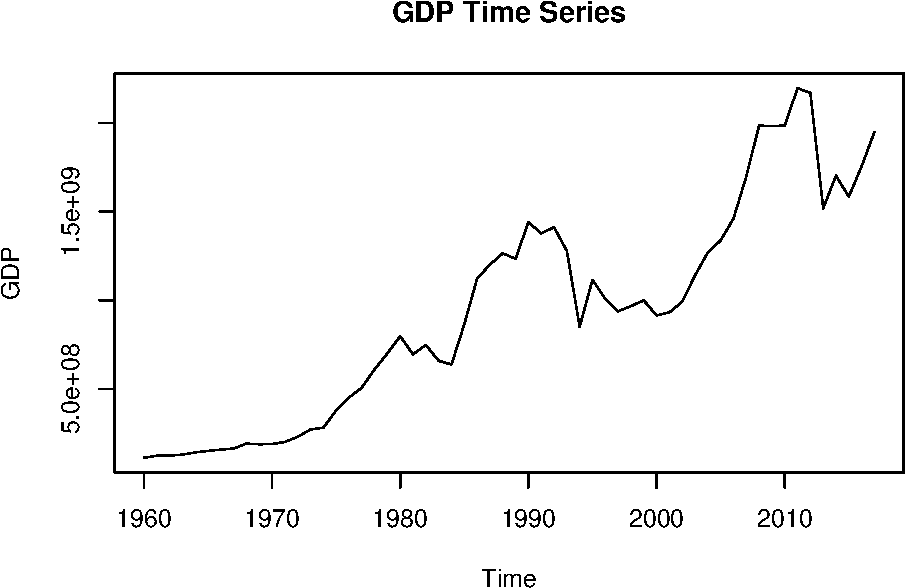
\includegraphics[keepaspectratio]{final_GDP_files/figure-latex/unnamed-chunk-3-1.pdf}}

Summary: - GDP time series has upward trend, this shows this is
non-stationary - It has peaks around every 10 year: 1980, 1990, 2010

\section{Transform}\label{transform}

\begin{Shaded}
\begin{Highlighting}[]
\CommentTok{\# Box{-}Cox transform GDP}
\NormalTok{lambda }\OtherTok{\textless{}{-}} \FunctionTok{BoxCox.lambda}\NormalTok{(gdp\_ts)}
\NormalTok{boxcox\_gdp\_ts }\OtherTok{\textless{}{-}} \FunctionTok{BoxCox}\NormalTok{(gdp\_ts, lambda)}
\FunctionTok{ts.plot}\NormalTok{(boxcox\_gdp\_ts, }\AttributeTok{main =} \FunctionTok{paste}\NormalTok{(}\StringTok{"Box{-}Cox Transformed GDP (lambda ="}\NormalTok{, }\FunctionTok{round}\NormalTok{(lambda, }\DecValTok{3}\NormalTok{), }\StringTok{")"}\NormalTok{), }\AttributeTok{ylab =} \StringTok{"Transformed GDP"}\NormalTok{)}
\end{Highlighting}
\end{Shaded}

\pandocbounded{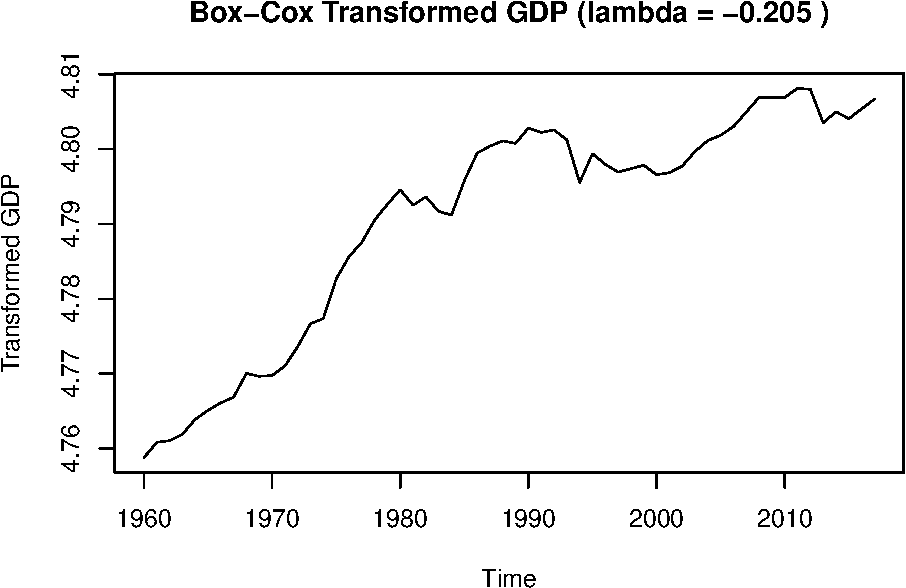
\includegraphics[keepaspectratio]{final_GDP_files/figure-latex/unnamed-chunk-4-1.pdf}}

We tried log, but residuals not normal.

\section{Differencing GDP}\label{differencing-gdp}

\begin{Shaded}
\begin{Highlighting}[]
\NormalTok{diff\_gdp\_bc }\OtherTok{\textless{}{-}} \FunctionTok{diff}\NormalTok{(boxcox\_gdp\_ts)}

\CommentTok{\# Plot differenced Box{-}Cox GDP}
\FunctionTok{ts.plot}\NormalTok{(diff\_gdp\_bc, }\AttributeTok{main=}\StringTok{"Differenced Box{-}Cox Transformed GDP Time Series"}\NormalTok{, }\AttributeTok{ylab=}\StringTok{"Transformed GDP"}\NormalTok{)}
\end{Highlighting}
\end{Shaded}

\pandocbounded{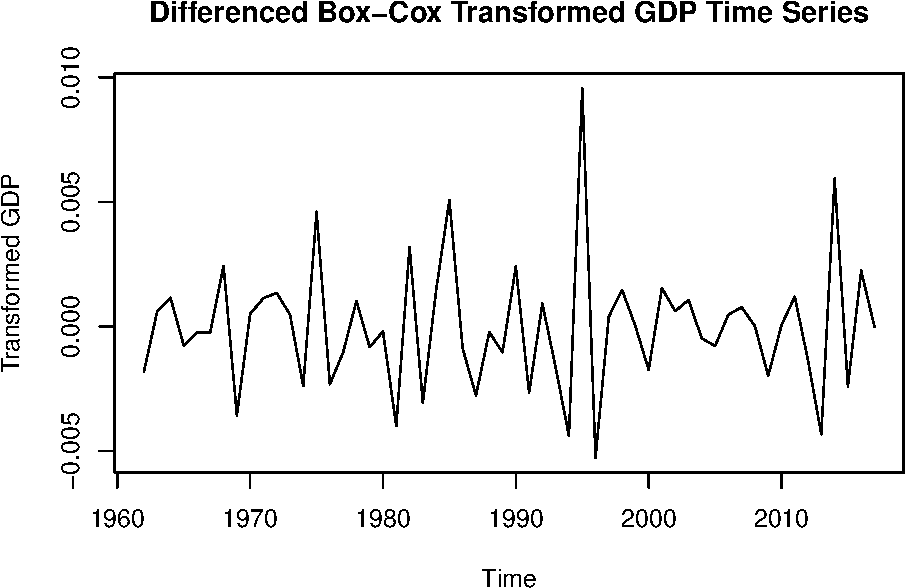
\includegraphics[keepaspectratio]{final_GDP_files/figure-latex/unnamed-chunk-5-1.pdf}}

\section{ACF / PACF plots}\label{acf-pacf-plots}

\begin{Shaded}
\begin{Highlighting}[]
\CommentTok{\# ACF and PACF of the transformed and differenced series}
\FunctionTok{par}\NormalTok{(}\AttributeTok{mfrow =} \FunctionTok{c}\NormalTok{(}\DecValTok{1}\NormalTok{, }\DecValTok{2}\NormalTok{))}
\FunctionTok{Acf}\NormalTok{(diff\_gdp\_bc, }\AttributeTok{main =} \StringTok{"ACF of Transformed + Differenced Series"}\NormalTok{)}
\FunctionTok{Pacf}\NormalTok{(diff\_gdp\_bc, }\AttributeTok{main =} \StringTok{"PACF of Transformed + Differenced Series"}\NormalTok{)}
\end{Highlighting}
\end{Shaded}

\pandocbounded{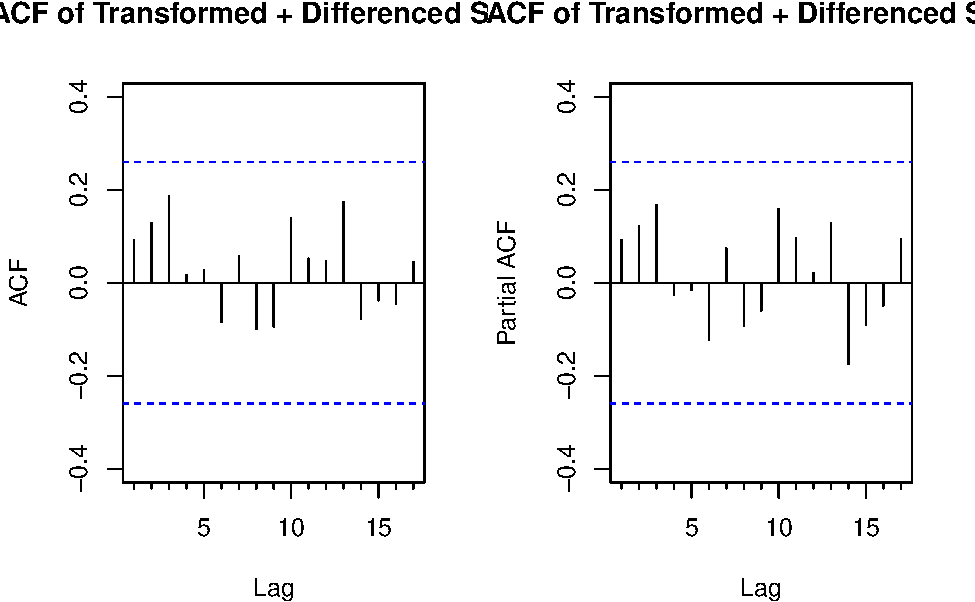
\includegraphics[keepaspectratio]{final_GDP_files/figure-latex/unnamed-chunk-6-1.pdf}}

\begin{Shaded}
\begin{Highlighting}[]
\FunctionTok{par}\NormalTok{(}\AttributeTok{mfrow =} \FunctionTok{c}\NormalTok{(}\DecValTok{1}\NormalTok{, }\DecValTok{1}\NormalTok{))}
\end{Highlighting}
\end{Shaded}

\section{Modeling}\label{modeling}

\begin{Shaded}
\begin{Highlighting}[]
\CommentTok{\# Central African Republic GDP ARIMA Model}
\CommentTok{\# Author: Om C}

\CommentTok{\# Diagnostics on chosen model}
\NormalTok{final\_model }\OtherTok{\textless{}{-}} \FunctionTok{Arima}\NormalTok{(boxcox\_gdp\_ts, }\AttributeTok{order =} \FunctionTok{c}\NormalTok{(}\DecValTok{0}\NormalTok{,}\DecValTok{1}\NormalTok{,}\DecValTok{0}\NormalTok{), }\AttributeTok{method =} \StringTok{"ML"}\NormalTok{)}
\FunctionTok{print}\NormalTok{(final\_model)}
\end{Highlighting}
\end{Shaded}

\begin{verbatim}
## Series: boxcox_gdp_ts 
## ARIMA(0,1,0) 
## 
## sigma^2 = 4.727e-06:  log likelihood = 271.1
## AIC=-540.2   AICc=-540.12   BIC=-538.15
\end{verbatim}

\begin{Shaded}
\begin{Highlighting}[]
\NormalTok{residuals\_final }\OtherTok{\textless{}{-}} \FunctionTok{residuals}\NormalTok{(final\_model)}

\CommentTok{\# Residual ACF and PACF for final model}
\FunctionTok{par}\NormalTok{(}\AttributeTok{mfrow =} \FunctionTok{c}\NormalTok{(}\DecValTok{1}\NormalTok{, }\DecValTok{2}\NormalTok{))  }\CommentTok{\# Side{-}by{-}side layout}
\FunctionTok{acf}\NormalTok{(residuals\_final, }\AttributeTok{main =} \StringTok{"ACF of Final Model Residuals"}\NormalTok{)}
\FunctionTok{pacf}\NormalTok{(residuals\_final, }\AttributeTok{main =} \StringTok{"PACF of Final Model Residuals"}\NormalTok{)}
\end{Highlighting}
\end{Shaded}

\pandocbounded{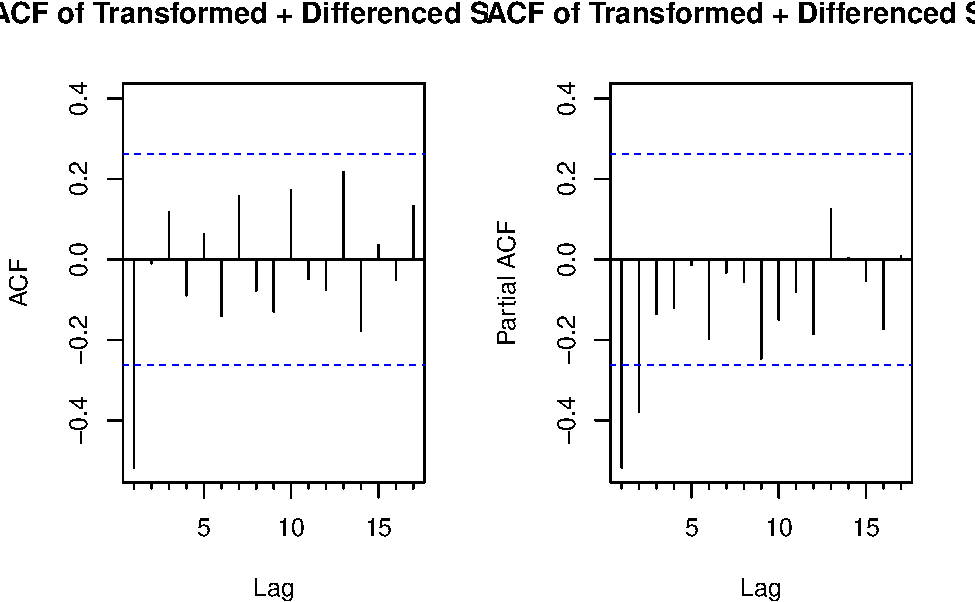
\includegraphics[keepaspectratio]{final_GDP_files/figure-latex/unnamed-chunk-7-1.pdf}}

\begin{Shaded}
\begin{Highlighting}[]
\FunctionTok{par}\NormalTok{(}\AttributeTok{mfrow =} \FunctionTok{c}\NormalTok{(}\DecValTok{1}\NormalTok{, }\DecValTok{1}\NormalTok{))  }\CommentTok{\# Reset layout}

\CommentTok{\# Diagnostic Tests (Simplified)}
\FunctionTok{cat}\NormalTok{(}\StringTok{"}\SpecialCharTok{\textbackslash{}n}\StringTok{Diagnostic Tests (Simplified):}\SpecialCharTok{\textbackslash{}n}\StringTok{"}\NormalTok{)}
\end{Highlighting}
\end{Shaded}

\begin{verbatim}
## 
## Diagnostic Tests (Simplified):
\end{verbatim}

\begin{Shaded}
\begin{Highlighting}[]
\CommentTok{\# 1. Portmanteau (Ljung{-}Box) Test for Autocorrelation}
\NormalTok{ljung }\OtherTok{\textless{}{-}} \FunctionTok{Box.test}\NormalTok{(residuals\_final, }\AttributeTok{lag =} \DecValTok{10}\NormalTok{, }\AttributeTok{type =} \StringTok{"Ljung{-}Box"}\NormalTok{)}
\FunctionTok{cat}\NormalTok{(}\StringTok{"Ljung{-}Box test p{-}value:"}\NormalTok{, }\FunctionTok{round}\NormalTok{(ljung}\SpecialCharTok{$}\NormalTok{p.value, }\DecValTok{4}\NormalTok{), }
    \FunctionTok{ifelse}\NormalTok{(ljung}\SpecialCharTok{$}\NormalTok{p.value }\SpecialCharTok{\textgreater{}} \FloatTok{0.05}\NormalTok{, }\StringTok{"(PASS {-} residuals approx white noise)"}\NormalTok{, }\StringTok{"(FAIL)"}\NormalTok{), }\StringTok{"}\SpecialCharTok{\textbackslash{}n}\StringTok{"}\NormalTok{)}
\end{Highlighting}
\end{Shaded}

\begin{verbatim}
## Ljung-Box test p-value: 0.8095 (PASS - residuals approx white noise)
\end{verbatim}

\begin{Shaded}
\begin{Highlighting}[]
\CommentTok{\# 2. Shapiro{-}Wilk Test for Normality}
\CommentTok{\# this does not violate model assumptions, but it violates confidence interval assumptions}
\NormalTok{shapiro }\OtherTok{\textless{}{-}} \FunctionTok{shapiro.test}\NormalTok{(residuals\_final)}
\FunctionTok{cat}\NormalTok{(}\StringTok{"Shapiro{-}Wilk test p{-}value:"}\NormalTok{, }\FunctionTok{round}\NormalTok{(shapiro}\SpecialCharTok{$}\NormalTok{p.value, }\DecValTok{4}\NormalTok{), }
    \FunctionTok{ifelse}\NormalTok{(shapiro}\SpecialCharTok{$}\NormalTok{p.value }\SpecialCharTok{\textgreater{}} \FloatTok{0.05}\NormalTok{, }\StringTok{"(PASS {-} approx. normal residuals)"}\NormalTok{, }\StringTok{"(FAIL)"}\NormalTok{), }\StringTok{"}\SpecialCharTok{\textbackslash{}n}\StringTok{"}\NormalTok{)}
\end{Highlighting}
\end{Shaded}

\begin{verbatim}
## Shapiro-Wilk test p-value: 0.0449 (FAIL)
\end{verbatim}

\begin{Shaded}
\begin{Highlighting}[]
\CommentTok{\# STEP 3: Model Comparison}
\NormalTok{models }\OtherTok{\textless{}{-}} \FunctionTok{list}\NormalTok{(}
  \StringTok{"ARIMA(0,1,0)"} \OtherTok{=} \FunctionTok{c}\NormalTok{(}\DecValTok{0}\NormalTok{,}\DecValTok{1}\NormalTok{,}\DecValTok{0}\NormalTok{), }\CommentTok{\# This implies a random walk, which is obviously an underfit for our model}
  \StringTok{"ARIMA(1,1,0)"} \OtherTok{=} \FunctionTok{c}\NormalTok{(}\DecValTok{1}\NormalTok{,}\DecValTok{1}\NormalTok{,}\DecValTok{0}\NormalTok{),}
  \StringTok{"ARIMA(0,1,1)"} \OtherTok{=} \FunctionTok{c}\NormalTok{(}\DecValTok{0}\NormalTok{,}\DecValTok{1}\NormalTok{,}\DecValTok{1}\NormalTok{),}
  \StringTok{"ARIMA(1,1,1)"} \OtherTok{=} \FunctionTok{c}\NormalTok{(}\DecValTok{1}\NormalTok{,}\DecValTok{1}\NormalTok{,}\DecValTok{1}\NormalTok{),}
  \StringTok{"ARIMA(2,1,0)"} \OtherTok{=} \FunctionTok{c}\NormalTok{(}\DecValTok{2}\NormalTok{,}\DecValTok{1}\NormalTok{,}\DecValTok{0}\NormalTok{),}
  \StringTok{"ARIMA(2,1,1)"} \OtherTok{=} \FunctionTok{c}\NormalTok{(}\DecValTok{2}\NormalTok{,}\DecValTok{1}\NormalTok{,}\DecValTok{1}\NormalTok{),}
  \StringTok{"ARIMA(2,1,2)"} \OtherTok{=} \FunctionTok{c}\NormalTok{(}\DecValTok{2}\NormalTok{,}\DecValTok{1}\NormalTok{,}\DecValTok{2}\NormalTok{),}
  \StringTok{"ARIMA(1,1,2)"} \OtherTok{=} \FunctionTok{c}\NormalTok{(}\DecValTok{1}\NormalTok{,}\DecValTok{1}\NormalTok{,}\DecValTok{2}\NormalTok{),}
  \StringTok{"ARIMA(0,1,2)"} \OtherTok{=} \FunctionTok{c}\NormalTok{(}\DecValTok{0}\NormalTok{,}\DecValTok{1}\NormalTok{,}\DecValTok{2}\NormalTok{)}
\NormalTok{)}
\NormalTok{results }\OtherTok{\textless{}{-}} \FunctionTok{data.frame}\NormalTok{(}\AttributeTok{Model=}\FunctionTok{character}\NormalTok{(), }\AttributeTok{AIC=}\FunctionTok{numeric}\NormalTok{(), }\AttributeTok{BIC=}\FunctionTok{numeric}\NormalTok{(), }
                     \AttributeTok{Ljung\_Box\_p=}\FunctionTok{numeric}\NormalTok{(), }\AttributeTok{stringsAsFactors=}\ConstantTok{FALSE}\NormalTok{)}

\ControlFlowTok{for}\NormalTok{(i }\ControlFlowTok{in} \DecValTok{1}\SpecialCharTok{:}\FunctionTok{length}\NormalTok{(models)) \{}
\NormalTok{  fit }\OtherTok{\textless{}{-}} \FunctionTok{Arima}\NormalTok{(boxcox\_gdp\_ts, }\AttributeTok{order =}\NormalTok{ models[[i]], }\AttributeTok{method =} \StringTok{"ML"}\NormalTok{)}
\NormalTok{  ljung\_p }\OtherTok{\textless{}{-}} \FunctionTok{Box.test}\NormalTok{(}\FunctionTok{residuals}\NormalTok{(fit), }\AttributeTok{lag =} \DecValTok{10}\NormalTok{, }\AttributeTok{type =} \StringTok{"Ljung{-}Box"}\NormalTok{)}\SpecialCharTok{$}\NormalTok{p.value}
\NormalTok{  results }\OtherTok{\textless{}{-}} \FunctionTok{rbind}\NormalTok{(results, }\FunctionTok{data.frame}\NormalTok{(}
    \AttributeTok{Model =} \FunctionTok{names}\NormalTok{(models)[i],}
    \AttributeTok{AIC =}\NormalTok{ fit}\SpecialCharTok{$}\NormalTok{aic,}
    \AttributeTok{BIC =} \FunctionTok{BIC}\NormalTok{(fit),}
    \AttributeTok{Ljung\_Box\_p =}\NormalTok{ ljung\_p}
\NormalTok{  ))}
\NormalTok{\}}
\FunctionTok{print}\NormalTok{(results)}
\end{Highlighting}
\end{Shaded}

\begin{verbatim}
##          Model       AIC       BIC Ljung_Box_p
## 1 ARIMA(0,1,0) -540.1976 -538.1545   0.8094629
## 2 ARIMA(1,1,0) -541.3535 -537.2674   0.7596909
## 3 ARIMA(0,1,1) -540.4525 -536.3664   0.8245419
## 4 ARIMA(1,1,1) -545.1549 -539.0258   0.8881498
## 5 ARIMA(2,1,0) -542.1543 -536.0251   0.7249147
## 6 ARIMA(2,1,1) -543.1641 -534.9919   0.8832207
## 7 ARIMA(2,1,2) -543.9988 -533.7835   0.9470827
## 8 ARIMA(1,1,2) -543.1627 -534.9904   0.8840160
## 9 ARIMA(0,1,2) -540.1068 -533.9777   0.7867186
\end{verbatim}

\begin{Shaded}
\begin{Highlighting}[]
\CommentTok{\# If we inspect the BIC too, the one with min AIC is likely to also have the min BIC}
\FunctionTok{cat}\NormalTok{(}\StringTok{"}\SpecialCharTok{\textbackslash{}n}\StringTok{Best model by AIC:"}\NormalTok{, results}\SpecialCharTok{$}\NormalTok{Model[}\FunctionTok{which.min}\NormalTok{(results}\SpecialCharTok{$}\NormalTok{AIC)], }\StringTok{"}\SpecialCharTok{\textbackslash{}n}\StringTok{"}\NormalTok{)}
\end{Highlighting}
\end{Shaded}

\begin{verbatim}
## 
## Best model by AIC: ARIMA(1,1,1)
\end{verbatim}

\begin{Shaded}
\begin{Highlighting}[]
\CommentTok{\# STEP 4: Final Model and Diagnostics}
\NormalTok{final\_model }\OtherTok{\textless{}{-}} \FunctionTok{Arima}\NormalTok{(boxcox\_gdp\_ts, }\AttributeTok{order =} \FunctionTok{c}\NormalTok{(}\DecValTok{1}\NormalTok{,}\DecValTok{1}\NormalTok{,}\DecValTok{1}\NormalTok{), }\AttributeTok{method =} \StringTok{"ML"}\NormalTok{)}
\FunctionTok{print}\NormalTok{(final\_model)}
\end{Highlighting}
\end{Shaded}

\begin{verbatim}
## Series: boxcox_gdp_ts 
## ARIMA(1,1,1) 
## 
## Coefficients:
##          ar1      ma1
##       0.9603  -0.8459
## s.e.  0.0808   0.1707
## 
## sigma^2 = 4.215e-06:  log likelihood = 275.58
## AIC=-545.15   AICc=-544.7   BIC=-539.03
\end{verbatim}

\begin{Shaded}
\begin{Highlighting}[]
\NormalTok{residuals\_final }\OtherTok{\textless{}{-}} \FunctionTok{residuals}\NormalTok{(final\_model)}

\CommentTok{\# Residual ACF and PACF for final model}
\FunctionTok{par}\NormalTok{(}\AttributeTok{mfrow =} \FunctionTok{c}\NormalTok{(}\DecValTok{1}\NormalTok{, }\DecValTok{2}\NormalTok{))  }\CommentTok{\# Side{-}by{-}side layout}
\FunctionTok{acf}\NormalTok{(residuals\_final, }\AttributeTok{main =} \StringTok{"ACF of Final Model Residuals"}\NormalTok{)}
\FunctionTok{pacf}\NormalTok{(residuals\_final, }\AttributeTok{main =} \StringTok{"PACF of Final Model Residuals"}\NormalTok{)}
\end{Highlighting}
\end{Shaded}

\pandocbounded{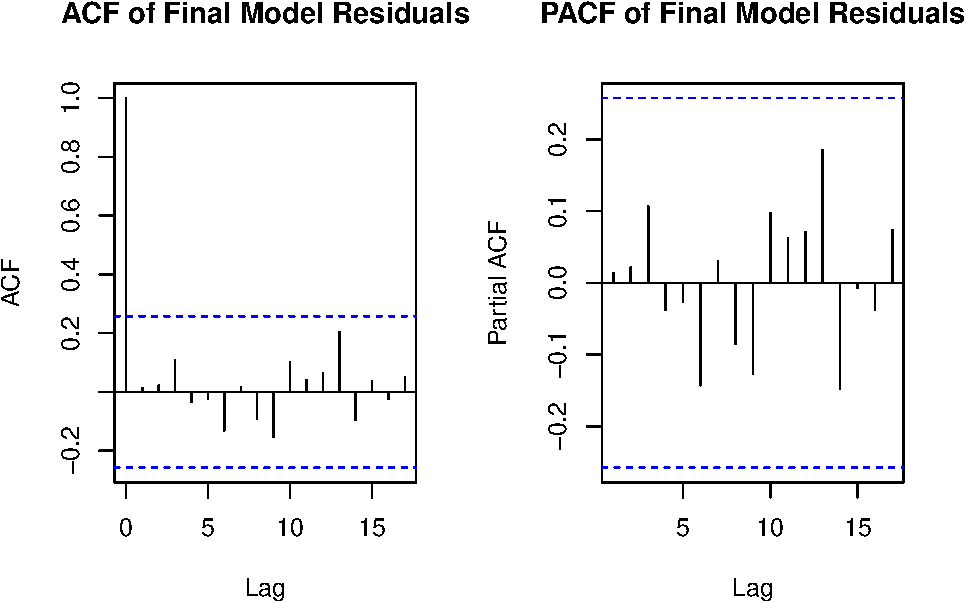
\includegraphics[keepaspectratio]{final_GDP_files/figure-latex/unnamed-chunk-7-2.pdf}}

\begin{Shaded}
\begin{Highlighting}[]
\FunctionTok{par}\NormalTok{(}\AttributeTok{mfrow =} \FunctionTok{c}\NormalTok{(}\DecValTok{1}\NormalTok{, }\DecValTok{1}\NormalTok{))  }\CommentTok{\# Reset layout}

\FunctionTok{cat}\NormalTok{(}\StringTok{"}\SpecialCharTok{\textbackslash{}n}\StringTok{Diagnostic Tests:}\SpecialCharTok{\textbackslash{}n}\StringTok{"}\NormalTok{)}
\end{Highlighting}
\end{Shaded}

\begin{verbatim}
## 
## Diagnostic Tests:
\end{verbatim}

\begin{Shaded}
\begin{Highlighting}[]
\CommentTok{\# 1. Ljung{-}Box test}
\NormalTok{ljung }\OtherTok{\textless{}{-}} \FunctionTok{Box.test}\NormalTok{(residuals\_final, }\AttributeTok{lag =} \DecValTok{10}\NormalTok{, }\AttributeTok{type =} \StringTok{"Ljung{-}Box"}\NormalTok{)}
\FunctionTok{cat}\NormalTok{(}\StringTok{"Ljung{-}Box test p{-}value:"}\NormalTok{, }\FunctionTok{round}\NormalTok{(ljung}\SpecialCharTok{$}\NormalTok{p.value, }\DecValTok{4}\NormalTok{), }
    \FunctionTok{ifelse}\NormalTok{(ljung}\SpecialCharTok{$}\NormalTok{p.value }\SpecialCharTok{\textgreater{}} \FloatTok{0.05}\NormalTok{, }\StringTok{"(PASS)"}\NormalTok{, }\StringTok{"(FAIL)"}\NormalTok{), }\StringTok{"}\SpecialCharTok{\textbackslash{}n}\StringTok{"}\NormalTok{)}
\end{Highlighting}
\end{Shaded}

\begin{verbatim}
## Ljung-Box test p-value: 0.8881 (PASS)
\end{verbatim}

\begin{Shaded}
\begin{Highlighting}[]
\CommentTok{\# 2. Normality test}
\CommentTok{\# this does not violate model assumptions, but it violates confidence interval assumptions}
\NormalTok{shapiro }\OtherTok{\textless{}{-}} \FunctionTok{shapiro.test}\NormalTok{(residuals\_final)}
\FunctionTok{cat}\NormalTok{(}\StringTok{"Shapiro{-}Wilk test p{-}value:"}\NormalTok{, }\FunctionTok{round}\NormalTok{(shapiro}\SpecialCharTok{$}\NormalTok{p.value, }\DecValTok{4}\NormalTok{), }
    \FunctionTok{ifelse}\NormalTok{(shapiro}\SpecialCharTok{$}\NormalTok{p.value }\SpecialCharTok{\textgreater{}} \FloatTok{0.05}\NormalTok{, }\StringTok{"(PASS)"}\NormalTok{, }\StringTok{"(FAIL)"}\NormalTok{), }\StringTok{"}\SpecialCharTok{\textbackslash{}n}\StringTok{"}\NormalTok{)}
\end{Highlighting}
\end{Shaded}

\begin{verbatim}
## Shapiro-Wilk test p-value: 0.0288 (FAIL)
\end{verbatim}

\begin{Shaded}
\begin{Highlighting}[]
\CommentTok{\# 3. ARCH test}
\NormalTok{arch }\OtherTok{\textless{}{-}} \FunctionTok{Box.test}\NormalTok{(residuals\_final}\SpecialCharTok{\^{}}\DecValTok{2}\NormalTok{, }\AttributeTok{lag =} \DecValTok{5}\NormalTok{, }\AttributeTok{type =} \StringTok{"Ljung{-}Box"}\NormalTok{)}
\FunctionTok{cat}\NormalTok{(}\StringTok{"ARCH test p{-}value:"}\NormalTok{, }\FunctionTok{round}\NormalTok{(arch}\SpecialCharTok{$}\NormalTok{p.value, }\DecValTok{4}\NormalTok{), }
    \FunctionTok{ifelse}\NormalTok{(arch}\SpecialCharTok{$}\NormalTok{p.value }\SpecialCharTok{\textgreater{}} \FloatTok{0.05}\NormalTok{, }\StringTok{"(PASS)"}\NormalTok{, }\StringTok{"(FAIL)"}\NormalTok{), }\StringTok{"}\SpecialCharTok{\textbackslash{}n}\StringTok{"}\NormalTok{)}
\end{Highlighting}
\end{Shaded}

\begin{verbatim}
## ARCH test p-value: 0.6157 (PASS)
\end{verbatim}

\begin{Shaded}
\begin{Highlighting}[]
\FunctionTok{cat}\NormalTok{(}\StringTok{"}\SpecialCharTok{\textbackslash{}n}\StringTok{Slight non{-}normality detected but acceptable for ARIMA modeling}\SpecialCharTok{\textbackslash{}n}\StringTok{"}\NormalTok{)}
\end{Highlighting}
\end{Shaded}

\begin{verbatim}
## 
## Slight non-normality detected but acceptable for ARIMA modeling
\end{verbatim}

\begin{Shaded}
\begin{Highlighting}[]
\FunctionTok{cat}\NormalTok{(}\StringTok{"Q{-}Q plot shows approximate normality with minor tail deviations}\SpecialCharTok{\textbackslash{}n\textbackslash{}n}\StringTok{"}\NormalTok{)}
\end{Highlighting}
\end{Shaded}

\begin{verbatim}
## Q-Q plot shows approximate normality with minor tail deviations
\end{verbatim}

\begin{Shaded}
\begin{Highlighting}[]
\CommentTok{\# STEP 5: Forecast with Inverse Transformation}
\NormalTok{forecast\_result }\OtherTok{\textless{}{-}} \FunctionTok{forecast}\NormalTok{(final\_model, }\AttributeTok{h =} \DecValTok{3}\NormalTok{)}
\NormalTok{lambda }\OtherTok{\textless{}{-}} \FloatTok{0.1}
\CommentTok{\# Inverse Box{-}Cox transformation}
\NormalTok{forecast\_original }\OtherTok{\textless{}{-}}\NormalTok{ (lambda }\SpecialCharTok{*}\NormalTok{ forecast\_result}\SpecialCharTok{$}\NormalTok{mean }\SpecialCharTok{+} \DecValTok{1}\NormalTok{)}\SpecialCharTok{\^{}}\NormalTok{(}\DecValTok{1}\SpecialCharTok{/}\NormalTok{lambda)}
\NormalTok{lower\_original }\OtherTok{\textless{}{-}}\NormalTok{ (lambda }\SpecialCharTok{*}\NormalTok{ forecast\_result}\SpecialCharTok{$}\NormalTok{lower }\SpecialCharTok{+} \DecValTok{1}\NormalTok{)}\SpecialCharTok{\^{}}\NormalTok{(}\DecValTok{1}\SpecialCharTok{/}\NormalTok{lambda)}
\NormalTok{upper\_original }\OtherTok{\textless{}{-}}\NormalTok{ (lambda }\SpecialCharTok{*}\NormalTok{ forecast\_result}\SpecialCharTok{$}\NormalTok{upper }\SpecialCharTok{+} \DecValTok{1}\NormalTok{)}\SpecialCharTok{\^{}}\NormalTok{(}\DecValTok{1}\SpecialCharTok{/}\NormalTok{lambda)}
\FunctionTok{cat}\NormalTok{(}\StringTok{"1{-}step ahead forecast (original GDP scale):"}\NormalTok{, }\FunctionTok{round}\NormalTok{(forecast\_original[}\DecValTok{1}\NormalTok{], }\DecValTok{2}\NormalTok{), }\StringTok{"million USD}\SpecialCharTok{\textbackslash{}n}\StringTok{"}\NormalTok{)}
\end{Highlighting}
\end{Shaded}

\begin{verbatim}
## 1-step ahead forecast (original GDP scale): 50.66 million USD
\end{verbatim}

\begin{Shaded}
\begin{Highlighting}[]
\FunctionTok{cat}\NormalTok{(}\StringTok{"95\% prediction interval: ["}\NormalTok{, }\FunctionTok{round}\NormalTok{(lower\_original[}\DecValTok{1}\NormalTok{,}\DecValTok{2}\NormalTok{], }\DecValTok{2}\NormalTok{), }\StringTok{","}\NormalTok{, }
    \FunctionTok{round}\NormalTok{(upper\_original[}\DecValTok{1}\NormalTok{,}\DecValTok{2}\NormalTok{], }\DecValTok{2}\NormalTok{), }\StringTok{"] million USD}\SpecialCharTok{\textbackslash{}n\textbackslash{}n}\StringTok{"}\NormalTok{)}
\end{Highlighting}
\end{Shaded}

\begin{verbatim}
## 95% prediction interval: [ 50.52 , 50.8 ] million USD
\end{verbatim}

\begin{Shaded}
\begin{Highlighting}[]
\FunctionTok{cat}\NormalTok{(}\StringTok{"FINAL MODEL: ARIMA(0,1,0) for Box{-}Cox transformed GDP}\SpecialCharTok{\textbackslash{}n}\StringTok{"}\NormalTok{)}
\end{Highlighting}
\end{Shaded}

\begin{verbatim}
## FINAL MODEL: ARIMA(0,1,0) for Box-Cox transformed GDP
\end{verbatim}

\section{Forecasting the next 10 time
periods}\label{forecasting-the-next-10-time-periods}

\begin{Shaded}
\begin{Highlighting}[]
\FunctionTok{library}\NormalTok{(ggplot2)}
\FunctionTok{library}\NormalTok{(forecast)}

\NormalTok{forecast\_horizon }\OtherTok{\textless{}{-}} \DecValTok{10}
\NormalTok{forecast\_values }\OtherTok{\textless{}{-}} \FunctionTok{forecast}\NormalTok{(final\_model, }\AttributeTok{h =}\NormalTok{ forecast\_horizon)}

\CommentTok{\# Enable LaTeX rendering in plots}
\FunctionTok{par}\NormalTok{(}\AttributeTok{pty=}\StringTok{"m"}\NormalTok{) }\CommentTok{\# reset plot type if needed}
\FunctionTok{options}\NormalTok{(}\AttributeTok{repr.plot.width=}\DecValTok{7}\NormalTok{, }\AttributeTok{repr.plot.height=}\DecValTok{5}\NormalTok{)}
\CommentTok{\# Note: In R base plotting, LaTeX rendering is not native; ggplot2 with expression() or latex2exp can be used.}
\CommentTok{\# Here we set theme with theme\_minimal() and use expression for labels.}

\FunctionTok{autoplot}\NormalTok{(forecast\_values) }\SpecialCharTok{+}
  \FunctionTok{ggtitle}\NormalTok{(}\FunctionTok{expression}\NormalTok{(}\StringTok{"Forecast for GDP"}\NormalTok{)) }\SpecialCharTok{+}
  \FunctionTok{xlab}\NormalTok{(}\FunctionTok{expression}\NormalTok{(}\StringTok{"Year"}\NormalTok{)) }\SpecialCharTok{+}
  \FunctionTok{ylab}\NormalTok{(}\FunctionTok{expression}\NormalTok{(}\StringTok{"GDP"}\NormalTok{)) }\SpecialCharTok{+}
  \FunctionTok{theme\_minimal}\NormalTok{()}
\end{Highlighting}
\end{Shaded}

\pandocbounded{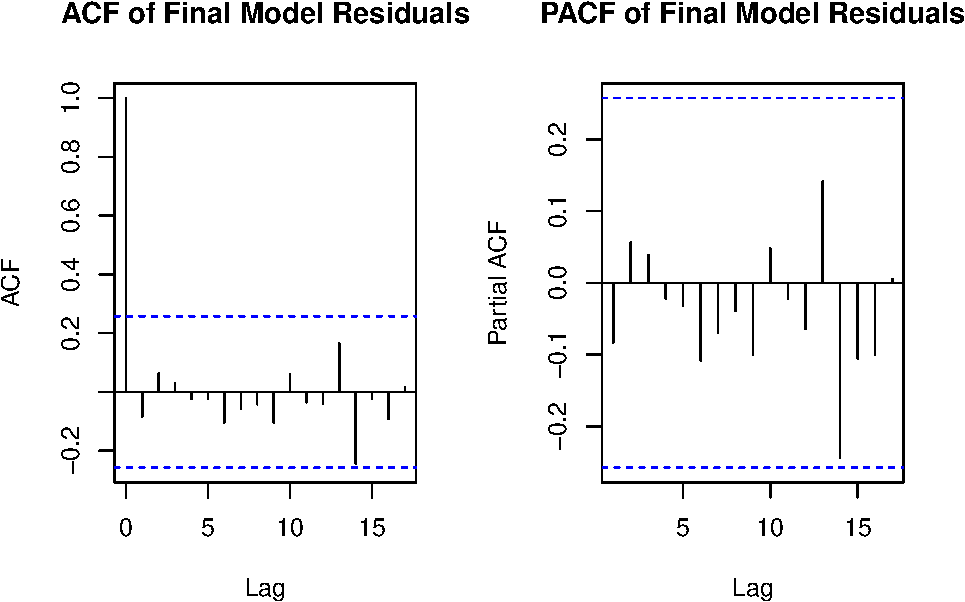
\includegraphics[keepaspectratio]{final_GDP_files/figure-latex/unnamed-chunk-8-1.pdf}}

\end{document}
